% !TEX root = ../presentation.tex
% !BIB program = biber
% !TEX program = xelatex

\section[A Retrospective Study on Machine Learning-Assisted Stroke Recognition for Medical Helpline Calls]{A Retrospective Study on Machine Learning-Assisted Stroke Recognition\\ for Medical Helpline Calls}


\begin{frame}
    \frametitle{Stroke}
    \begin{itemize}
        \item Stroke is a leading cause of disability and death worldwide \parencite{cite1,cite2,cite3}.
        \item Effective treatment is very time-sensitive. \parencite{cite4,cite5}.
        \item The gateway to ambulance transport and hospital admittance is through prehospital telehealth services.
        \item In the pre-hospital setting, the use of mobile stroke units has made it possible to deliver advanced treatment faster \parencite{cite6,cite7}.
        \item As the mobile stroke unit is only dispatched to patients with a suspected stroke, the impact of mobile stroke unit is directly influenced by accurate call-taker recognition of stroke \parencite{cite6,cite7}.
        \item Call-taker ability to rapidly and accurately recognize stroke is crucial in facilitating prompt care in both pre-hospital and in-hospital settings.
    \end{itemize}
\end{frame}


\begin{frame}
    \frametitle{Population selection and datasets}
    \begin{figure}
        \centering
        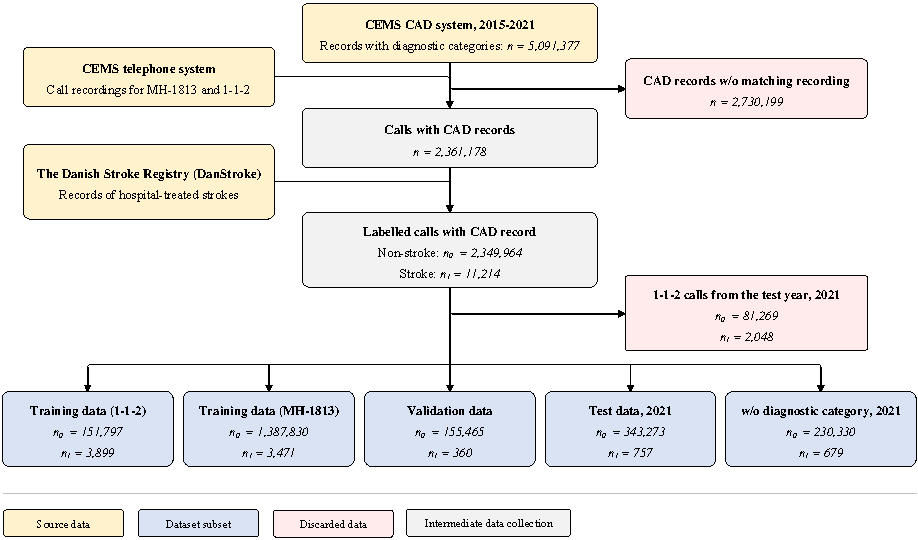
\includegraphics[width=0.62\paperwidth]{../graphics/paper_retrospective/data_flowchart.pdf}
    \end{figure}
\end{frame}


\begin{frame}
    \frametitle{Population characteristics}
    \begin{figure}
        \centering
        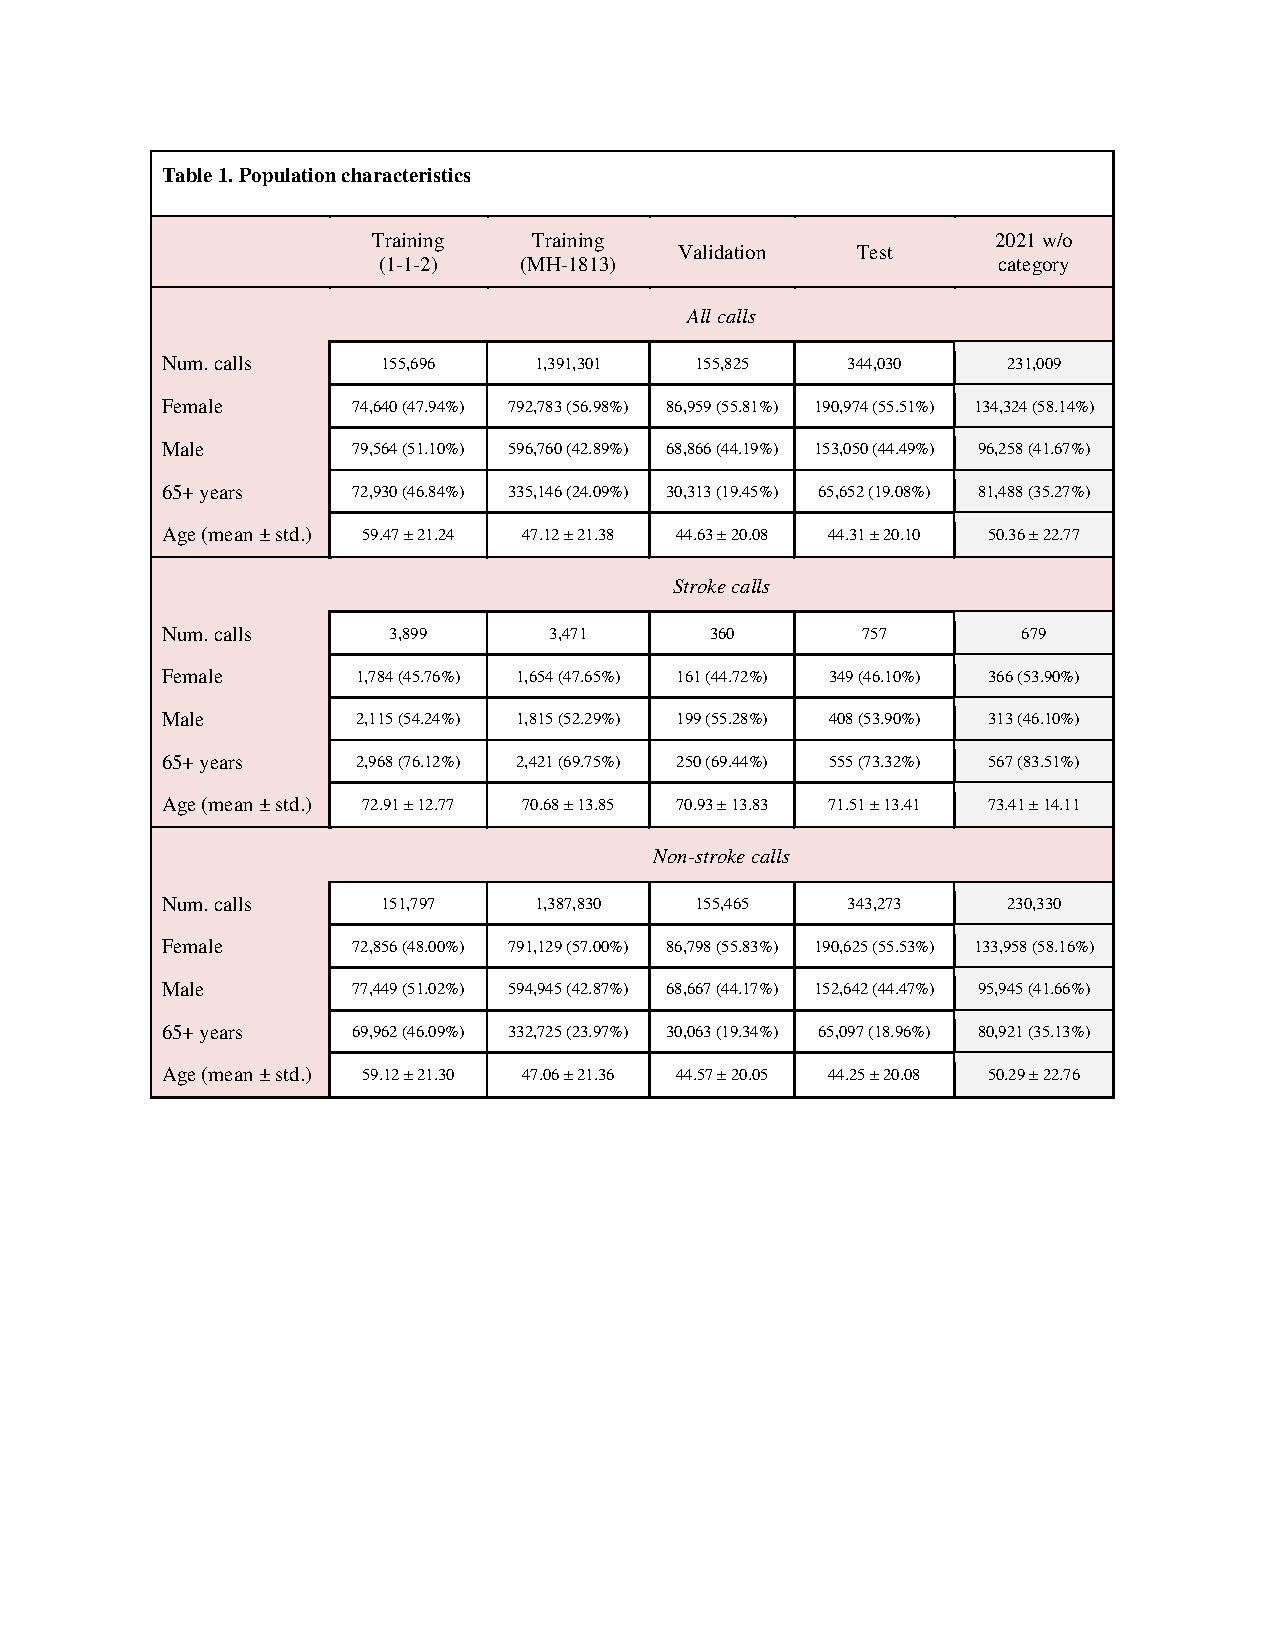
\includegraphics[width=0.3\paperwidth]{../graphics/paper_retrospective/table1.pdf}
    \end{figure}
\end{frame}


\begin{frame}
    \frametitle{Model design}
    \begin{figure}
        \centering
        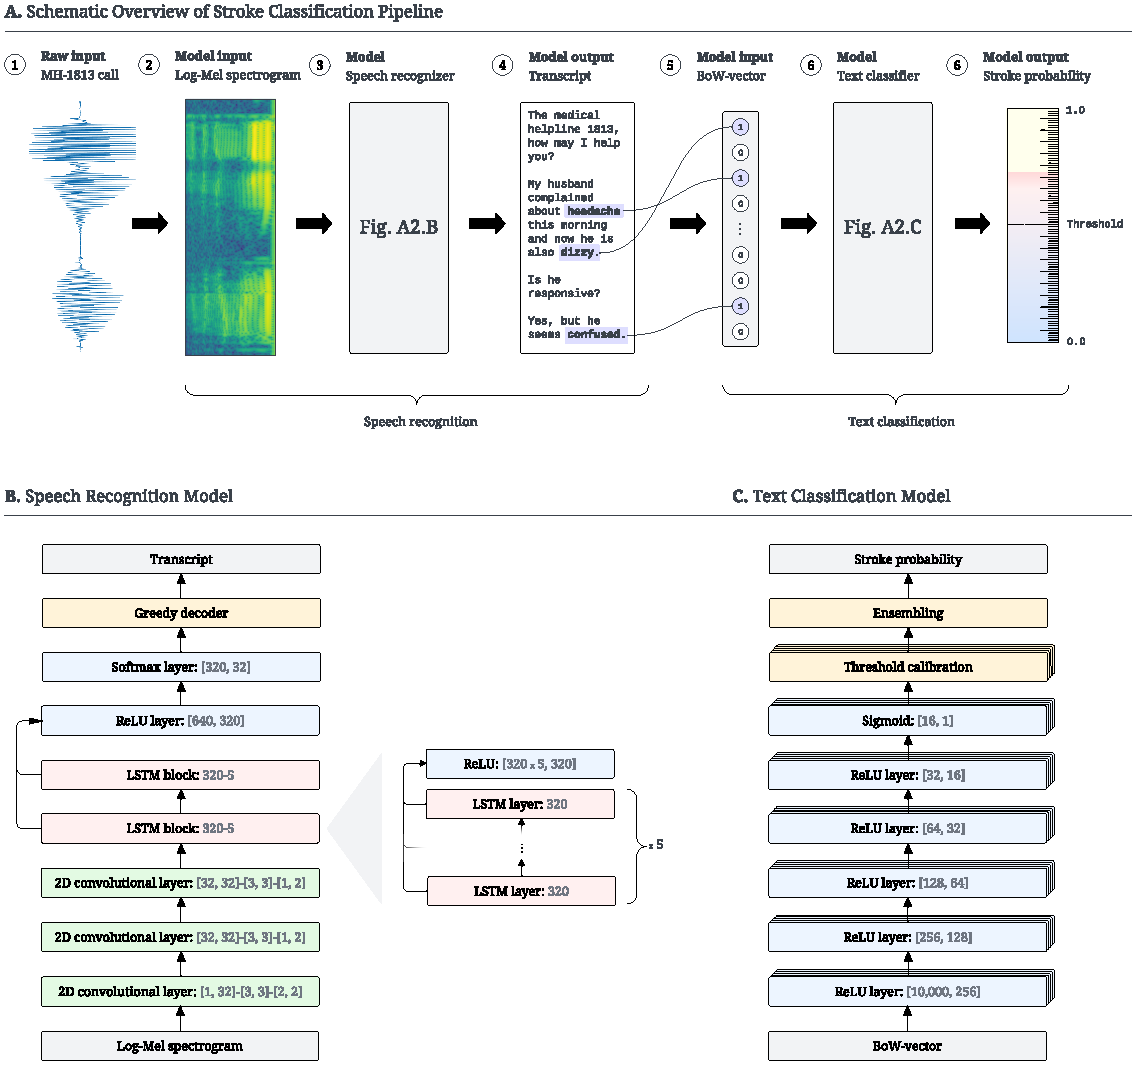
\includegraphics[width=0.40\paperwidth]{../graphics/paper_retrospective/model_sketch.pdf}
    \end{figure}
\end{frame}


\begin{frame}
    \frametitle{Model performance}
    \begin{figure}
        \centering
        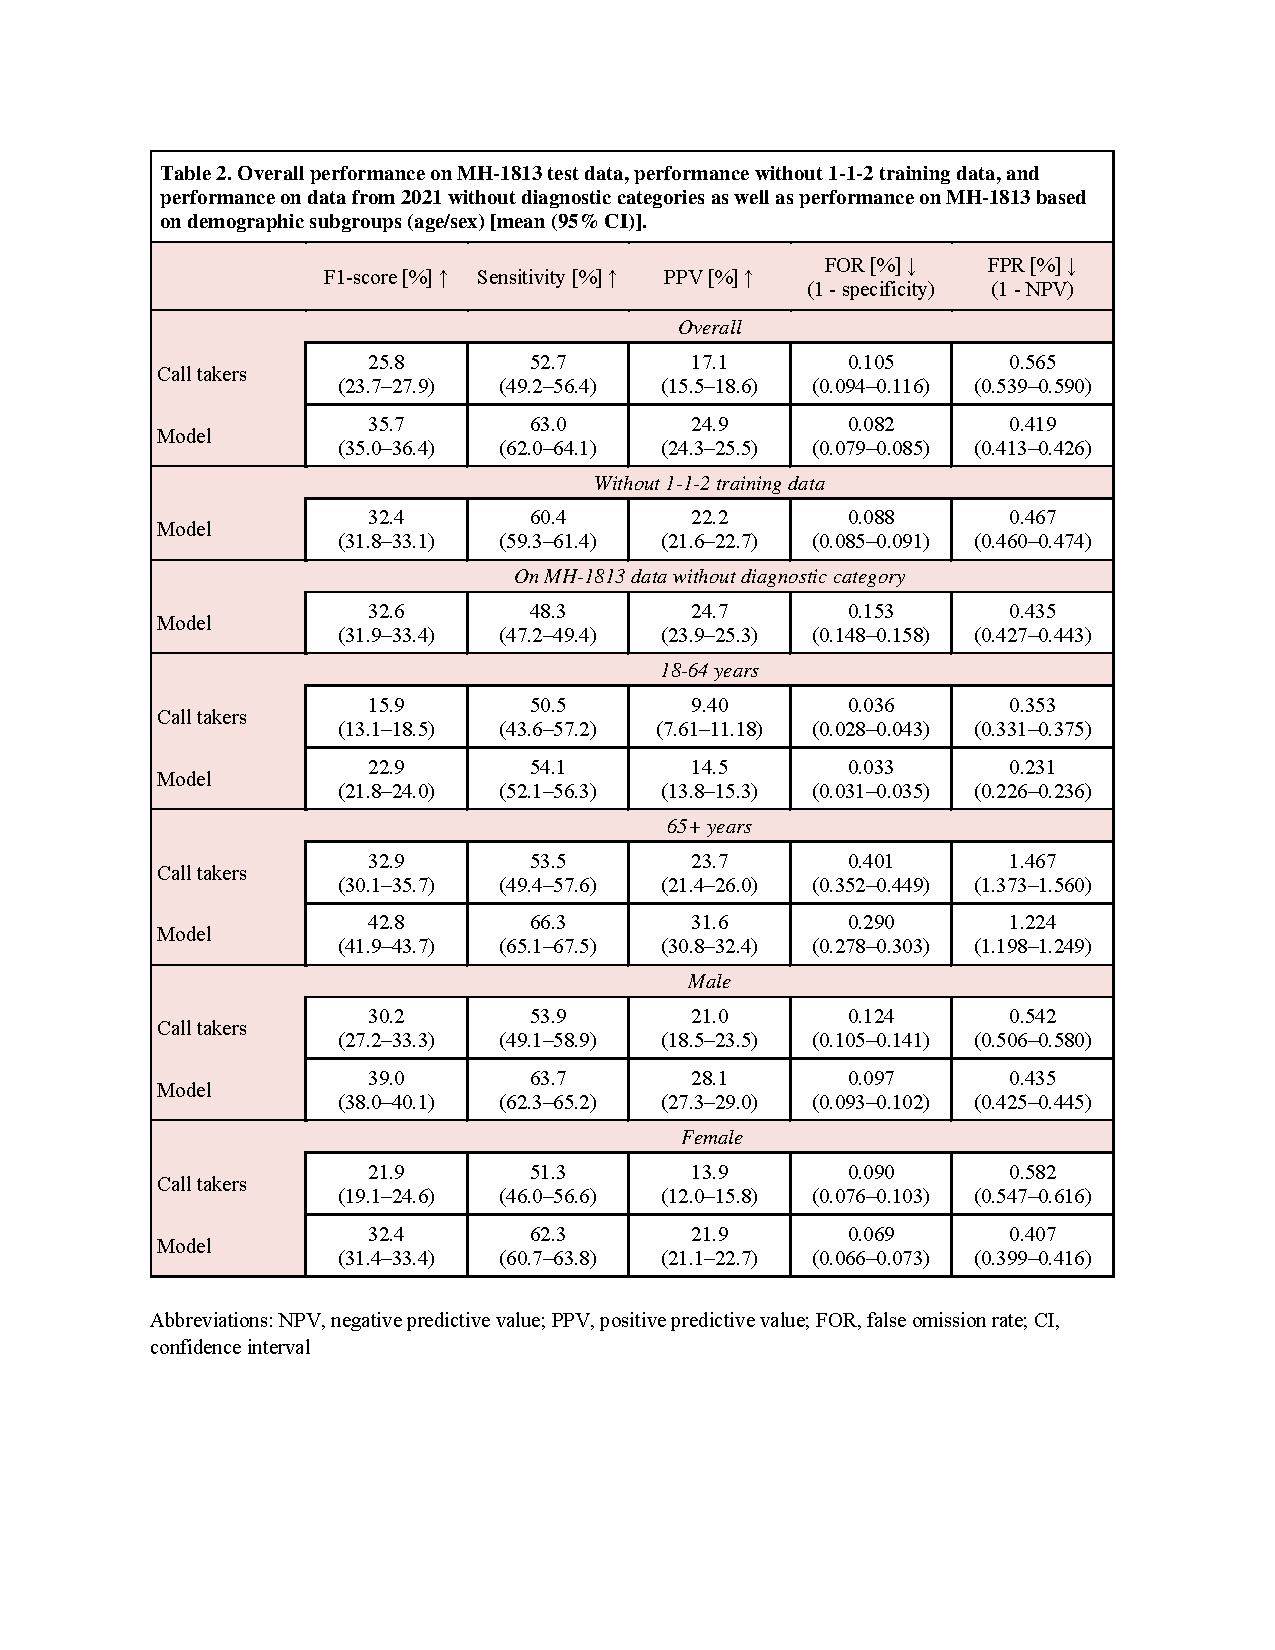
\includegraphics[width=0.3\paperwidth]{../graphics/paper_retrospective/table2.pdf}
    \end{figure}
\end{frame}


\begin{frame}
    \frametitle{Model performance}
    \begin{figure}
        \centering
        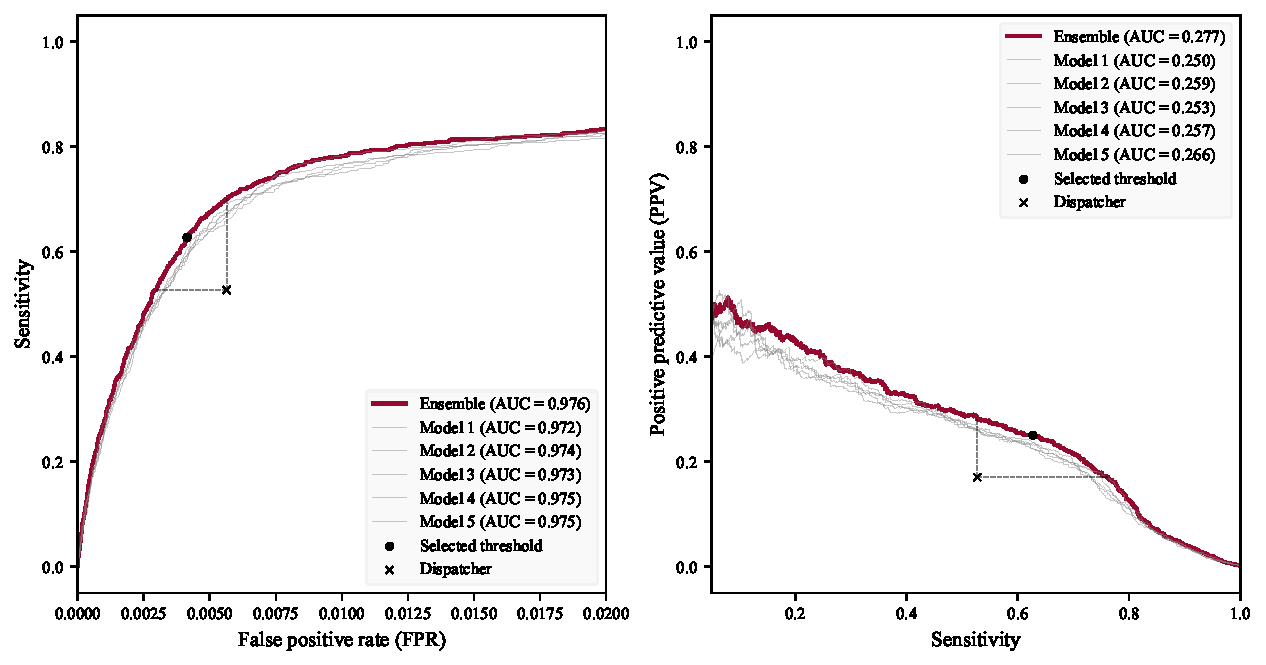
\includegraphics[width=0.65\paperwidth]{../graphics/paper_retrospective/figure1.pdf}
    \end{figure}
\end{frame}


\begin{frame}
    \frametitle{Model performance}
    \begin{figure}
        \centering
        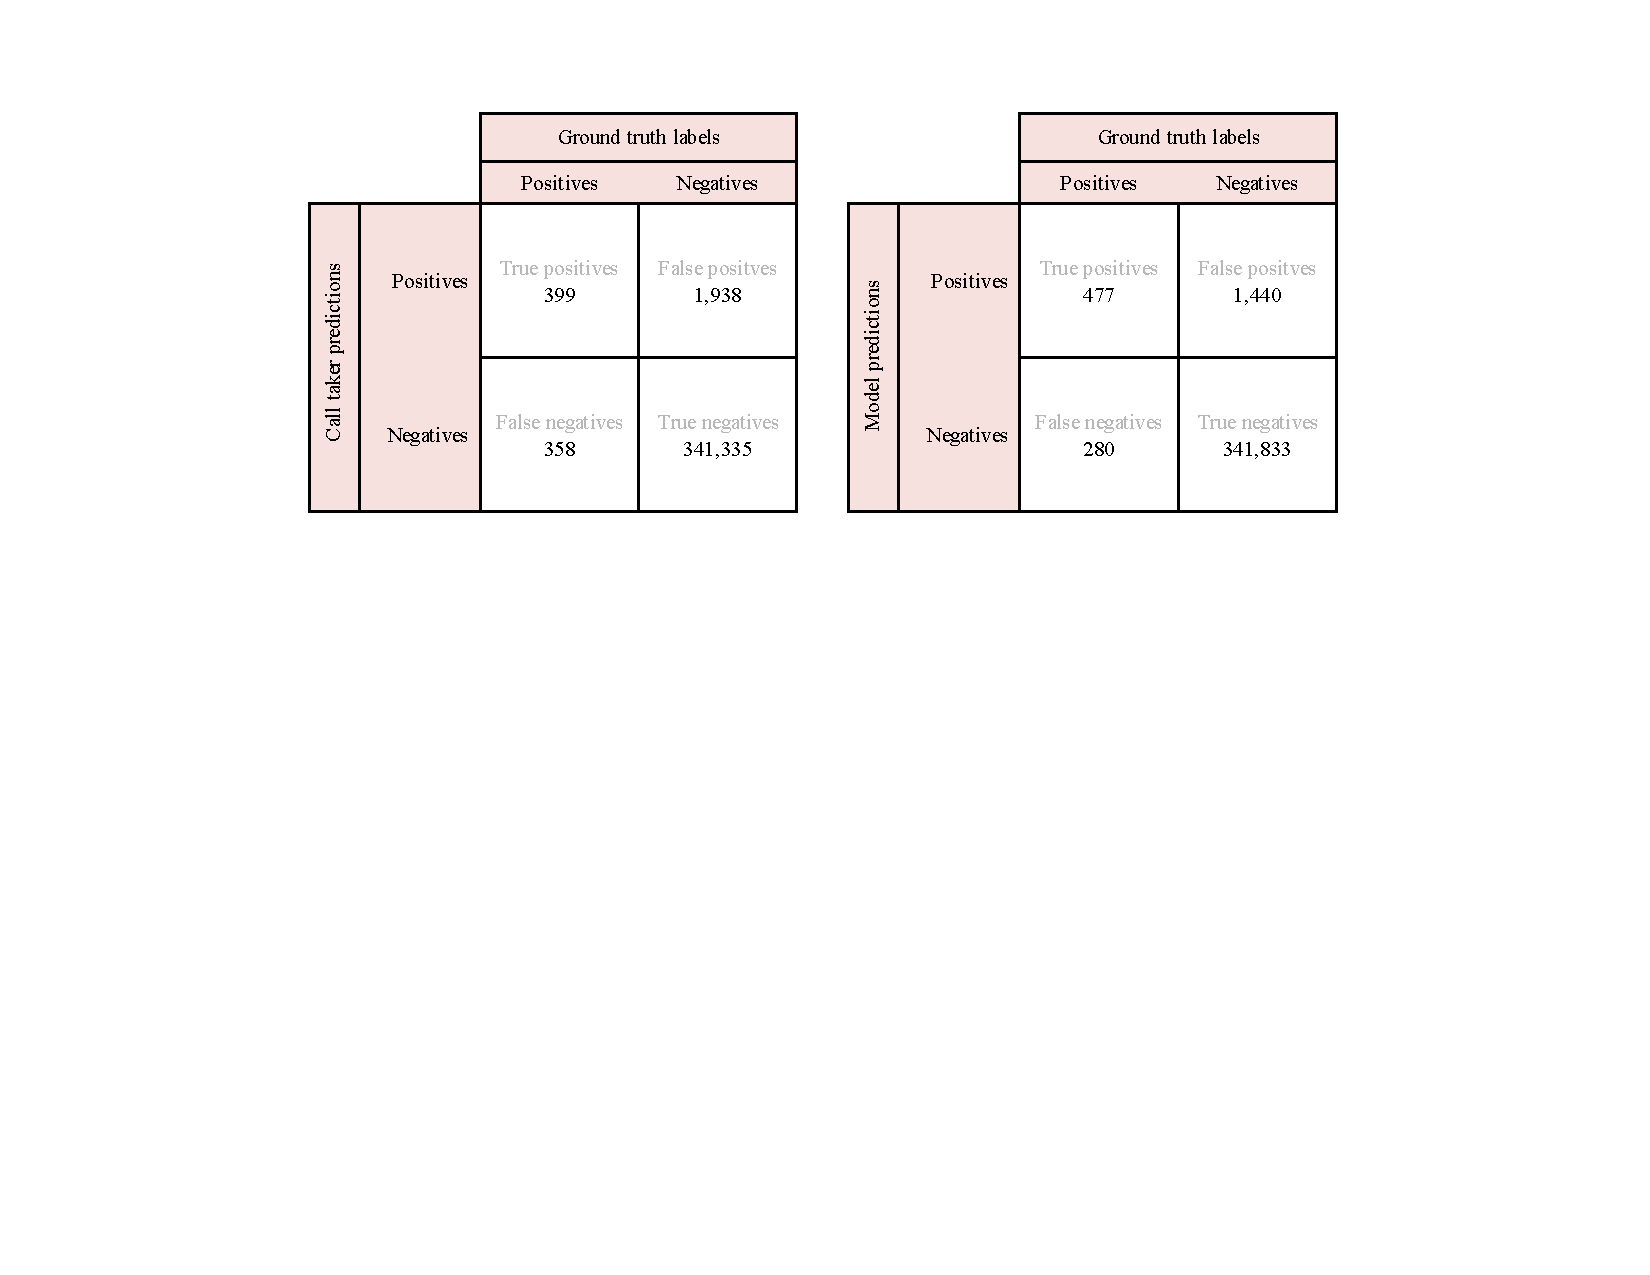
\includegraphics[width=0.95\paperwidth]{../graphics/paper_retrospective/figure2.pdf}
    \end{figure}
\end{frame}


\begin{frame}
    \frametitle{Which features are important?}
    \begin{figure}
        \centering
        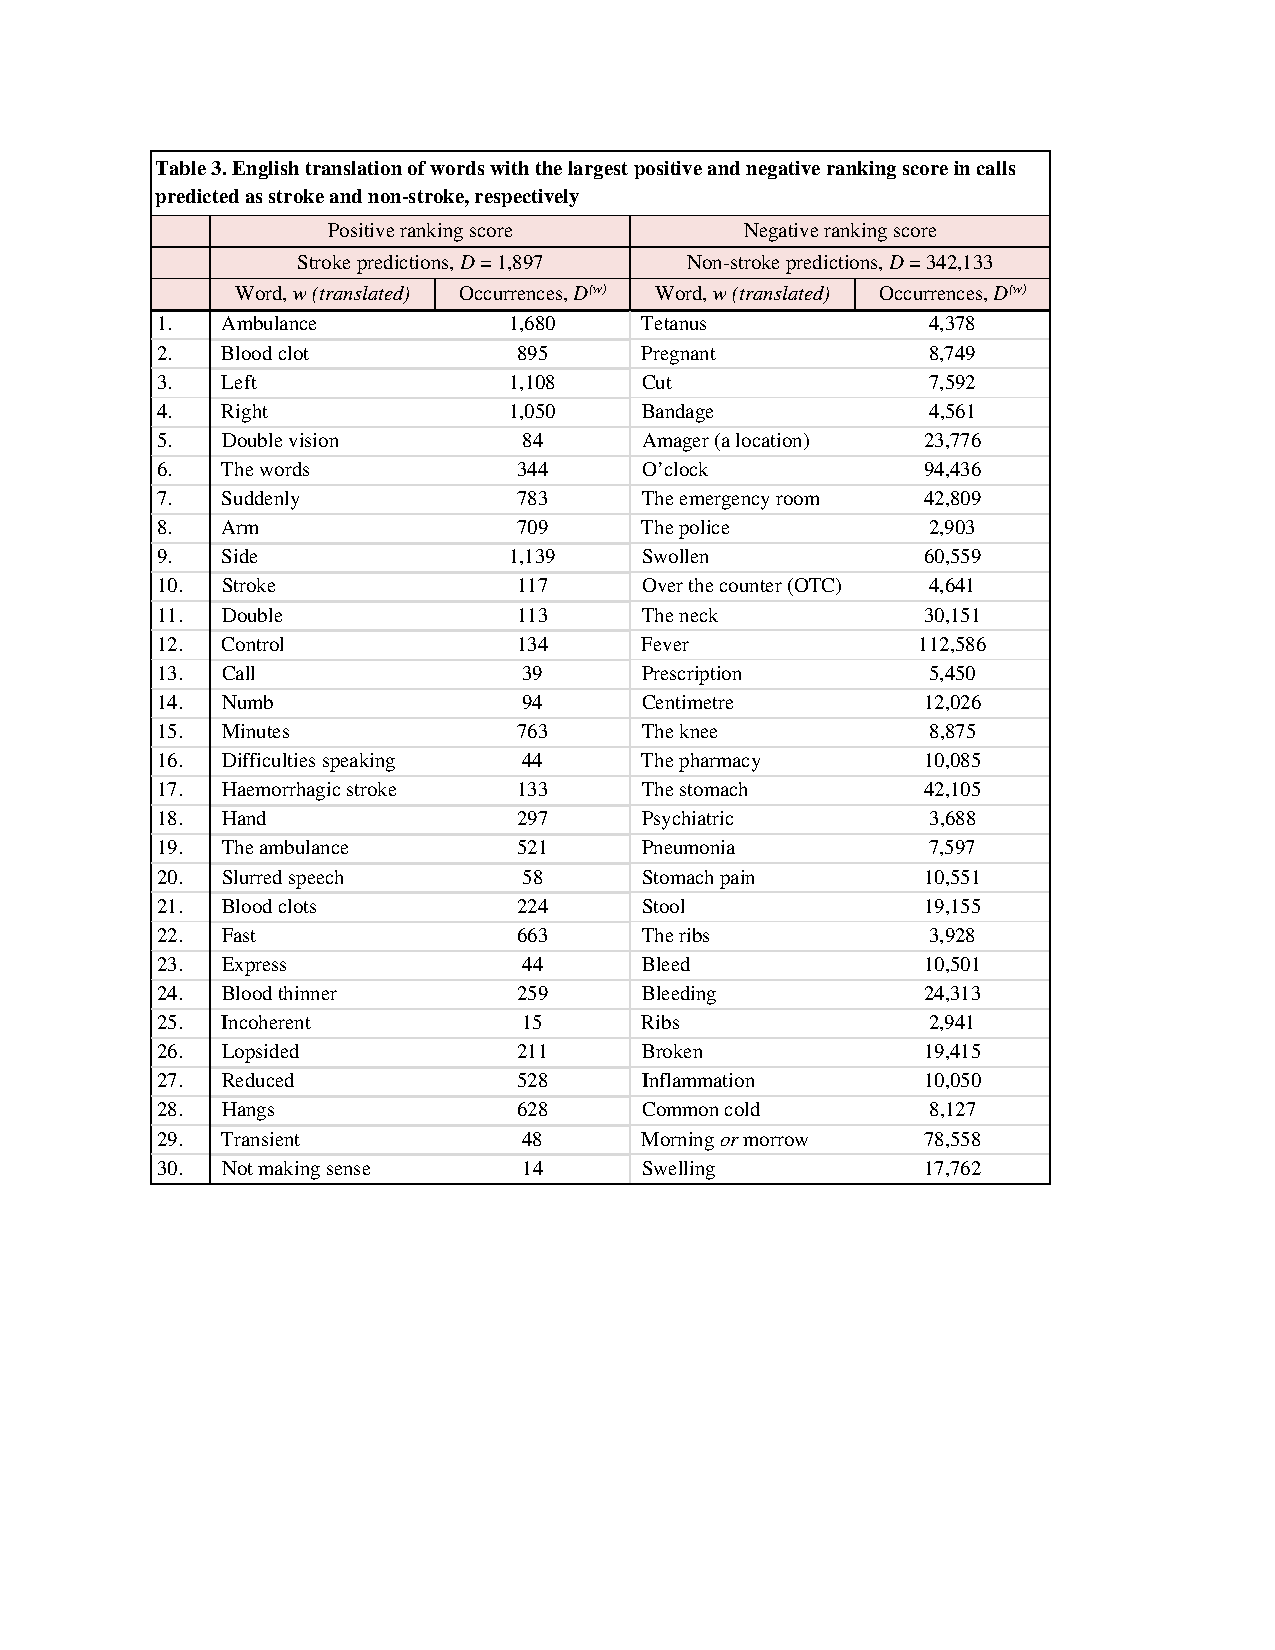
\includegraphics[width=0.4\paperwidth]{../graphics/paper_retrospective/table3.pdf}
    \end{figure}
\end{frame}


\begin{frame}
    \frametitle{Simulated prospective study}
    \begin{enumerate}
        \item[I.] {\color{dtured}When} is the model prediction presented to the call-taker?
        \begin{enumerate}
            \item[1.] Notify the call-taker of potential false positive or negative stroke cases after the call ends.
            \item[2.] Notify the call-taker of potential false positive or negative stroke cases during the call.
        \end{enumerate}
        \item[II.] {\color{dtured}How} does prediction influence the diagnostic code the call-taker assigns to the call?
        \begin{enumerate}[label=\Alph*.]
            \item[A.] Call-takers change any stroke prediction from negative to positive if the model predicts a positive (call-takers mirror model positives).
            \item[B.] Call-takers change any stroke prediction from positive to negative if the model predicts a negative (call-takers mirror model negatives).
        \end{enumerate}
    \end{enumerate}
        % %
        % Option 1 is identical to the method used in the main study. In option 2, predictions are made during the call based only on partial transcriptions. We implemented option 2 in such a manner that the model predicted every time 50 new words were transcribed and added to the transcript. A stroke positive was triggered only when three consecutive positive predictions were made (i.e., without intermediate negative stroke predictions). In other words, the sigmoid activation of the model had to remain above 0.5 for three consecutive predictions, for example, after 150, 200, and 250 words were transcribed.
        
        % As we can only assume how call takers are influenced by model predictions (II), precisely evaluating the hypothetical performance of call takers when supported by a machine learning framework is impossible. Furthermore, option 2 may influence the conversation, further complicating matters. Therefore, we report the results combining the call taker and the model under the following two assumptions:
        % %
\end{frame}


\begin{frame}
    \frametitle{Simulated prospective study}

    \begin{table}
        \centering
        % \caption{Overall performance of model, call-takers and simulated combinations of model and call-takers on MH-1813 test data.}
        % \label{tab_retrospective:tableA9}
        \resizebox*{0.98\textwidth}{!}{%
        \begin{tabular}{c|c|cc|cc|cc}
            \toprule
    
            Predictor & Call-taker & \multicolumn{2}{c|}{Model} & \multicolumn{4}{c}{Call-taker supported by the model (simulated)} \\
            \midrule
            When & - & After call & During call & After call & During call & After call & During call \\
            \midrule
            Method & - & 1.C & 2.C & 1.A & 1.B & 2.A & 2.B \\
            \midrule
    
            \makecell[l]{F1-score [\%] $\uparrow$}                   & \makecell[c]{25.8 \\ (23.7-27.9)} & \makecell[c]{35.7 \\ (35.0-36.4)} & \makecell[c]{33.1 \\ (32.4-33.7)} & \makecell[c]{28.9 \\ (28.3-29.5)} & \makecell[c]{33.3 \\ (32.5-34.1)} & \makecell[c]{27.6 \\ (27.0-28.1)} & \makecell[c]{32.7 \\ (31.8-33.5)} \\
            \midrule
            \makecell[l]{Sensitivity [\%] $\uparrow$}                & \makecell[c]{52.7 \\ (49.2-56.4)} & \makecell[c]{63.0 \\ (62.0-64.1)} & \makecell[c]{58.7 \\ (57.7-59.8)} & \makecell[c]{72.4 \\ (71.5-73.3)} & \makecell[c]{43.4 \\ (42.3-44.5)} & \makecell[c]{72.3 \\ (71.4-73.3)} & \makecell[c]{39.1 \\ (38.1-40.1)} \\
            \midrule
            \makecell[l]{PPV [\%] $\uparrow$}                        & \makecell[c]{17.1 \\ (15.5-18.6)} & \makecell[c]{24.9 \\ (24.3-25.5)} & \makecell[c]{23.0 \\ (22.5-23.6)} & \makecell[c]{18.0 \\ (17.6-18.4)} & \makecell[c]{27.0 \\ (26.3-27.8)} & \makecell[c]{17.0 \\ (16.7-17.4)} & \makecell[c]{28.1 \\ (27.3-28.9)} \\
            \midrule
            \makecell[l]{FOR [\%] $\downarrow$ \\ (1 - NPV)}         & \makecell[c]{0.105 \\ (0.094-0.116)} & \makecell[c]{0.082 \\ (0.079-0.085)} & \makecell[c]{0.091 \\ (0.088-0.094)} & \makecell[c]{0.061 \\ (0.059-0.064)} & \makecell[c]{0.125 \\ (0.121-0.129)} & \makecell[c]{0.061 \\ (0.059-0.064)} & \makecell[c]{0.134 \\ (0.131-0.138)} \\
            \midrule
            \makecell[l]{FPR [\%] $\downarrow$ \\ (1 - specificity)} & \makecell[c]{0.565 \\ (0.539-0.590)} & \makecell[c]{0.419 \\ (0.413-0.426)} & \makecell[c]{0.432 \\ (0.426-0.439)} & \makecell[c]{0.726 \\ (0.717-0.735)} & \makecell[c]{0.258 \\ (0.253-0.263)} & \makecell[c]{0.776 \\ (0.767-0.786)} & \makecell[c]{0.221 \\ (0.216-0.226)} \\
    
            \bottomrule
        \end{tabular}%
        }
    \end{table}

\end{frame}

% Stroke is a leading cause of disability and death worldwide \parencite{cite1,cite2,cite3}. Effective treatment is time-sensitive, and an optimal outcome is more likely when treatment is administered within the first four and a half hours from stroke onset \parencite{cite4,cite5}. The gateway to ambulance transport and hospital admittance is through prehospital telehealth services, including emergency medical call centers, nurse advice call lines, and out-of-hours health services. In the pre-hospital setting, the use of mobile stroke units has made it possible to deliver advanced treatment faster \parencite{cite6,cite7}. As the mobile stroke unit is only dispatched to patients with a suspected stroke, the impact of mobile stroke unit is directly influenced by accurate call-taker recognition of stroke \parencite{cite6,cite7}. Call-takers who can rapidly and accurately recognize stroke are therefore crucial in facilitating prompt care in both pre-hospital and in-hospital settings.

% Despite initiatives to improve stroke recognition \parencite{cite8,cite9}, approximately half of all patients with stroke do not receive the correct triage for their condition from call-takers \parencite{cite10,cite11,cite12}. Most initiatives aim to improve stroke recognition by call-takers via introducing more specific assessment tools \parencite{cite8,cite9} or providing specialized training \parencite{cite13}. Recent advances in machine learning technology might be applied to improve stroke recognition without requiring changes to the triaging approach, and machine learning aided identification of stroke has been suggested as a means of improving mobile stroke unit effectiveness \parencite{cite7}. Real-time feedback from a machine learning model can improve the recognition of out-of-hospital cardiac arrest \parencite{cite14,cite15}. Therefore, this study aimed to develop and assess the potential of machine learning in improving prehospital stroke recognition during medical helpline calls. 

% In this study, we use call recordings and registry data from the Copenhagen Emergency Medical Services (CEMS) and the Danish Stroke Registry (DanStroke) \parencite{cite16} from 2015 to 2020. We obtain call recordings from two call lines: the 1-1-2 emergency line and the medical helpline 1813 (MH-1813). We then fit a machine learning framework to classify medical helpline calls as stroke or non-stroke. Calls are first transcribed using an automatic speech recognition model and then categorized by a text classification model trained as an ensemble of five individual models. We compare the performance of the model with that of call-takers using MH-1813 data from 2021.

